\documentclass[10pt,english]{beamer}
%\documentclass[english,handout]{beamer} % For handouts
\input{../metropolis_preamble.tex}
\input{../macros.tex}
%\usepackage{extendedalt}
%\usepackage{animate} % Animations
%\usepackage{../lindsten}
%\usepackage{movie15}

\title{732G57 Maskininlärning för statistiker}
\subtitle{Föreläsning 5}
\date{}
\author{Josef Wilzén \\ IDA, Linköping University, Sweden}
\titlegraphic{\hfill
\includegraphics[height=1.2cm]{../LiU_primary_black.pdf}}
%\institute{Joint work with\dots}

\hypersetup{
  colorlinks=true, urlcolor=blue, linkcolor=red
}

%% MY DEF %%
\newcommand{\itm}[1]{\mathrm{Item}_{#1}}
\newcommand{\pausa}{\pause}
%\renewcommand{\pausa}{}


\newenvironment{nscenter}
 {\parskip=0pt\par\nopagebreak\centering}
 {\par\noindent\ignorespacesafterend}

\begin{document}

\maketitle

\begin{frame}{Dagens föreläsning}
    
    \begin{itemize}
        \item Linjära och icke-linjära modeller
        \item Trädmodeller
        \item Metoder för besultsträd
        \item Regularisering
    \end{itemize}

\end{frame}


\begin{frame}{Linjär regression till icke-linjär?}
    
    Förklarande variabler $\mathbf{X} = (x_1, x_2, \ldots, x_p)$ och respons $y$.

    Modellerear som $y = \mathbf{X}\beta$.

    Ett sätt att hantera icke-linjära samband är att transformera $\mathbb{X}$.

    Till exempel:
    \begin{itemize}
        \item Polynomregression
        \item Andra funktioner
        \item Interaktioner
        \item Stegfunktioner
        \item Diskretisering
    \end{itemize}

    Svårt att veta vilka transformationer man ska göra, svårt att transformera komplexa datastrukturer.

\end{frame}

\begin{frame}{Icke-linjära modeller}
    
    Maskininlärning har gett oss många olika metoder för att anpassa mer generella icke-linjära modeller.

    \begin{greenbox}
        Målet är att hitta "automatiska" transformationer av de förklarande variablerna.
    \end{greenbox}

    Ska kunna hantera många variabler av olika typer.

    Exempel:
    \begin{itemize}
         \item Splines
        \item Local regression
        \item Generalized additive models
        \item K-närmaste grannar
        \item Trädmodeller
        \item Neurala nätverk
        \item Support vector machines
        
    \end{itemize}

\end{frame}

\begin{frame}{Trädmodeller}
    \begin{greenbox}
        Idé: Dela upp variabelrummet i icke överlappande regioner (rektanglar), alla observationer i samma region har samma anpassade värde.
    \end{greenbox}

    Reglerna för att hitta en specifik region kan beskrivas i en trädstruktur (binärt träd) $\rightarrow$ kallas för trädmodeller.

    Skattning inom ett område sker oftast genom medelvärde eller typvärde.

    Hur delar vi upp variabelrummet på ett bra sätt?
\end{frame}

\begin{frame}{Besultsträd}
    \begin{columns}
        \begin{column}{0.5\textwidth}
           Ett träd består av:
           \begin{itemize}
            \item Rotnod (N1)
            \item Noder (N*)
            \item Löv/slutnoder (N4-N7)
            \item Regler (Cond.1-Cond.6)
            \item Varje löv har ett tilldelat klassvärde
           \end{itemize}
        \end{column}
        \begin{column}{0.5\textwidth}  %%<--- here
            \begin{center}
             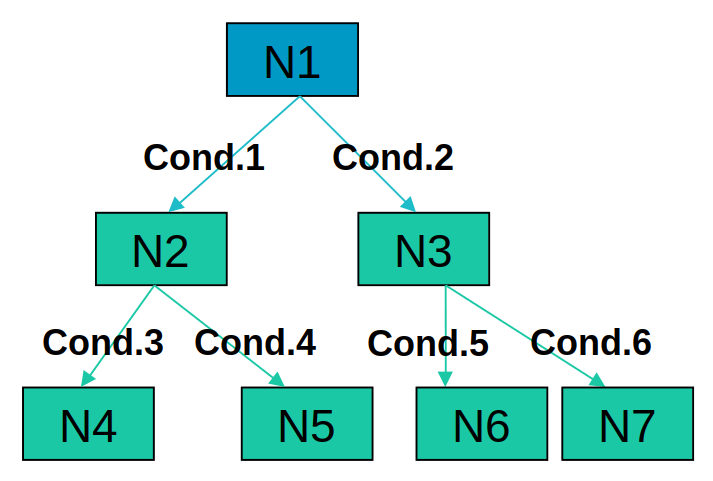
\includegraphics[width=\textwidth]{figs/tree1.png}
             \end{center}
        \end{column}
        \end{columns}
\end{frame}

\begin{frame}{Beslutsträd Exempel}
    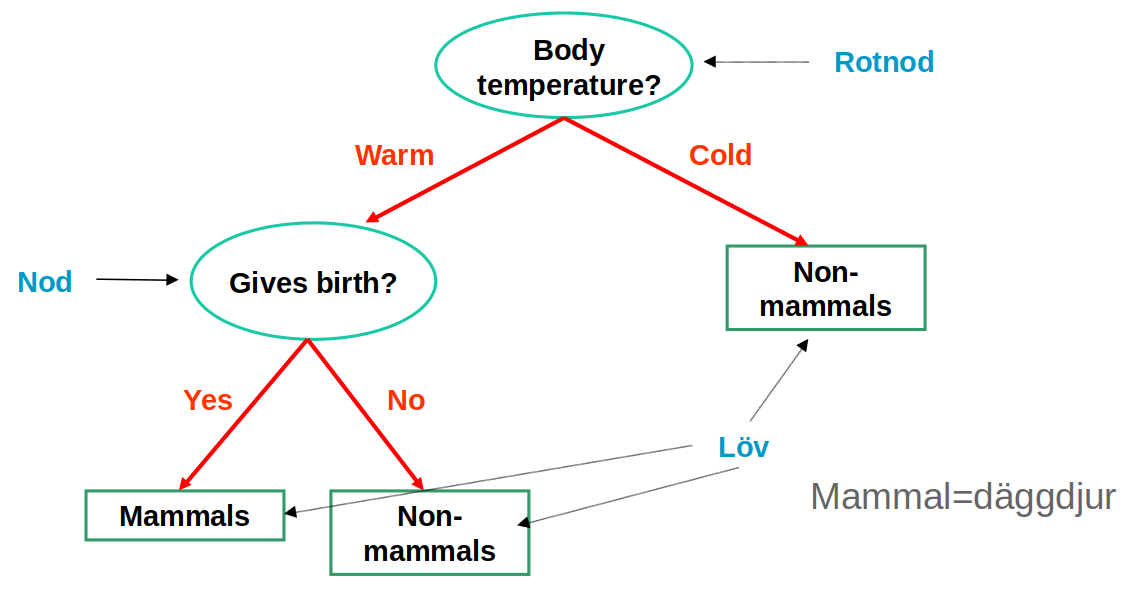
\includegraphics[width=\textwidth]{figs/tree2.png}
\end{frame}

\begin{frame}{Att bygga ett träd}
    \myheading{Hunt's algoritm}
    \begin{enumerate}
        \item Givet en nuvarande datamängd $D_t = \{(X_i, Y_i), i = 1,\ldots,n\}$ för den aktuella noden $t$.
        \item Om alla $Y_i$ är lika, markera $t$ som ett löv och ge värdet $Y_i$.
        \item Annars, använd en \myheading{testregel} för att dela upp $D_t$ i flera delar $D_{t_1}, \ldots, D_{t_k}$ och kör algoritmen (steg 1) för alla dessa noder.
    \end{enumerate}
    
    Denna approach kallas för \textit{recursive binary splitting}.
      
    \myheading{Testregler:} välj variabel, välj uppdelning
    \begin{description}
        \item[Binära attribut] Binär uppdelning
        \item[Nomiala attribut] Binär uppdelninig
        \item[Ordinala attribut] Uppdelning som bevarar attributsföljden
        \item[Intervall attribut] Uppdelning till icke-överlappande intervall
    \end{description}
\end{frame}

\begin{frame}{Att bygga ett träd - Exempel}

    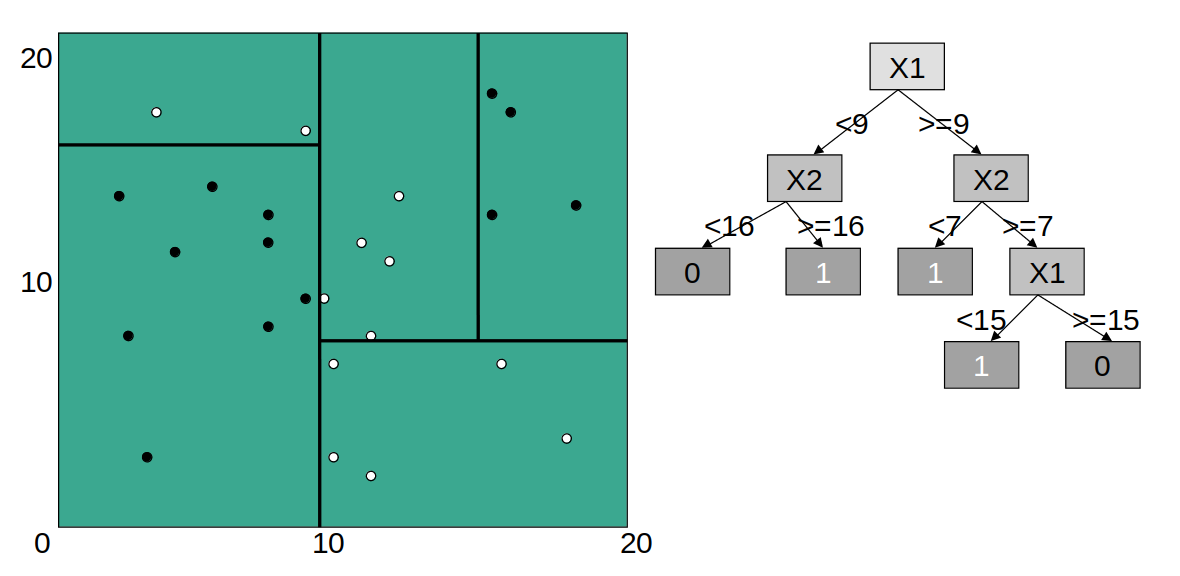
\includegraphics[width=\textwidth]{figs/tree3.png}
    
\end{frame}

\begin{frame}{Trädmodeller}
    
    Sammanfattninig:
    \begin{itemize}
        \item Idé: Dela upp observationerna för att separera klasser.
        \item Uppdelningen sker genom att jämföra testregler.
        \item För att avsluta processen:
        \begin{itemize}
            \item Dela upp tills alla observationer har samma klass
            \item Alt 1. Dela upp tills alla attribut är lika.
            \item Alt 2. Bestäm en regel för tidigt avslut.
        \end{itemize}
    \end{itemize}

\end{frame}

\begin{frame}{CART}
    Classification and Regression Trees (CART).

    I grunden Hunt's algoritm.

    Stöd för kontinuerliga och diskreta utfall.

    Optimering för att välja bästa splitten.
\end{frame}

\begin{frame}{CART - Regressionsträd}
    
    Att försöka minimera RSS över alla möjliga partitioneringar och funktionsvärden är orimligt.

    Istället kör vi med en girig algoritm, där vi vill hitta bästa variabeln $x_j$ och uppdelning $s$ genom att lösa följande problem:
    \begin{align*}
        \min_{j,s} \left[ \min_{c_1} \sum_{x_1 \in R_1(j,s)} (y_i - c_1)^2 + \min_{c_2} \sum_{x_i \in R_2(j,s)} (y_i - c_2)^2 \right], \\
        R_1(j,s) = \{x \mid x_j < s\} \qquad R_2(j,s) = \{x | x_j \geq s\},
    \end{align*}
    $c_1$ och $c_2$ skattas oftast som medelvärdet av respektive region.
    
    Finns effektiva algoritmer för att söka igenom bästa splittpunkten $s$ för alla förklarande variabler.
    
\end{frame}

\begin{frame}{CART - Regressionsträd}
    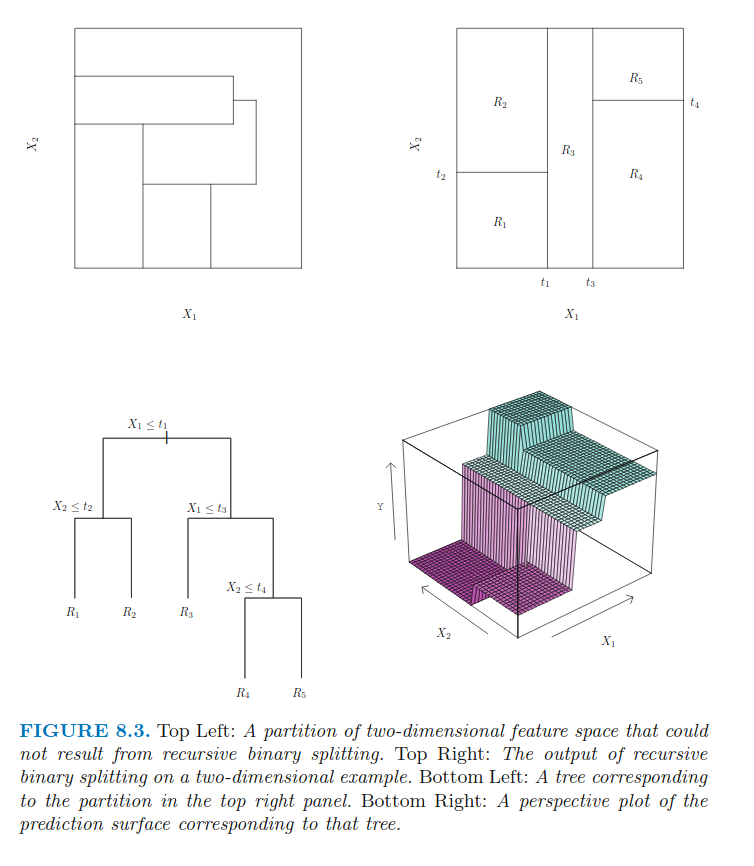
\includegraphics[width=0.68\textwidth]{figs/reg_tree_surface.png}
\end{frame}

\begin{frame}{CART - Regressionsträd}
   Exempel i R:
   
   
   \href{https://raw.githubusercontent.com/STIMALiU/732G57_ML/master/lectures/lecture5/tree_regression_example1.R}{Kod1}
   
   \href{https://raw.githubusercontent.com/STIMALiU/732G57_ML/master/lectures/lecture5/tree_regression_example2.R}{Kod2}
   
\end{frame}


\begin{frame}{CART - Klassificeringsträd}
    
    När det kommer till klassificering behöver vi ett nytt mått för att utvärdera om en regel är bra eller dålig.

    Låt $p_{m,k} = \frac{1}{s} \sum_{i : x_i \in R_m} \mathbb{I}_{y_i = k}$ vara proportionen av träningsdata i region $m$ som tillhör klass $k$.

    Kriterier för att välja regioner:
    \begin{description}
        \item[Felkvot] $E = 1 - \max_{k} (p_{m,k})$
        \item[Gini index] $G = \sum_{k} p_{m,k} ( 1 - p_{m,k}) = 1 - \sum_{k} p_{m,k}^2$
        \item[Cross-entropy] $D = - \sum_{k} p_{m,k} \log(p_{m,k})$   
    \end{description}

\end{frame}

\begin{frame}{CART - Klassificeringsträd}

    Välj nu den uppdelning som maximerar informationsvinsten
    \begin{align*}
        \Delta = I(\text{förälder}) - I(\text{barn}), \\
        \Delta = I(\text{förälder}) - \sum_{j} \frac{N(R_j)}{N} I(R_j),
    \end{align*}
    Där
    \begin{description}
        \item[$I(\cdot)$] är ditt valda mått (Felkvot, Gini, Entropy)
        \item[$N$] antal objekt i föräldranoden
        \item[$R_j$] är barnnod $j$
        \item[$N(R_j)$] antal objekt i barnnod $j$    
    \end{description}
    
\end{frame}

\begin{frame}{CART - Klassificeringsträd}

    Predikationer görs med majoritetsröstninig. Vi vill helst att alla observationer i ett löv ska ha samma klass.

    Vi stoppar utbyggnadet på samma sätt som i Hunt's algoritm.

    Entropy och Gini är bättre mått, de ger renare löv.

    Felkvoten används ofta för att utvärdera trädet på testdata.

    Trädmodeller överanpassar väldigt lätt. Vilket ger en hög varians på framtida testdata!
    
\end{frame}



\begin{frame}{Motverka överanpassning}

    Viktiga hyperparametrar:
    \begin{itemize}
      \item Trädets djup
      \item Minsta antal obs i en lövnod alt. minsta antal obs i en nod för att överväga en split av noden
    \end{itemize}

    Två olika sätt:
    \begin{description}
        \item[Förbeskärnining]
        \begin{itemize}
            \item Sluta expandera trädet när informationsvinsten är lägre än en vald tröskel.
            \item Kräv ett visst minsta antal obs i varje löv.
        \end{itemize}
        \item[Efterbeskärninig]
        \begin{itemize}
            \item Beskär ett helt utväxt träd, ersätt delträd med ett löv.
        \end{itemize}
    \end{description}
    
\end{frame}



\begin{frame}{Efterbeskärning}
    Använd CART för att ta växa fram ett stort träd $T_0$ på all träningsdata.

    För varje $\alpha \geq 0$ finns ett delträd $T \subset T_0$ som minimerar kostanden
    \begin{equation*}
        C_{\alpha}(T) = \sum_{R \in \text{Löv i T}} N(R) \cdot I(R) + \alpha |T|,
    \end{equation*} 
    där $|T|$ är antalet löv i $T$, $N(R_j)$ antal objekt i lövnod $j$. $I(\cdot)$ 
    är ditt valda utvärderingsmått

    Använd korsvalidering för att skatta $\alpha$, välj det som ger minst valideringsfel.

    Idén är lik LASSO.
\end{frame}



\begin{frame}{Regressionsträd med cost complexity pruning}
    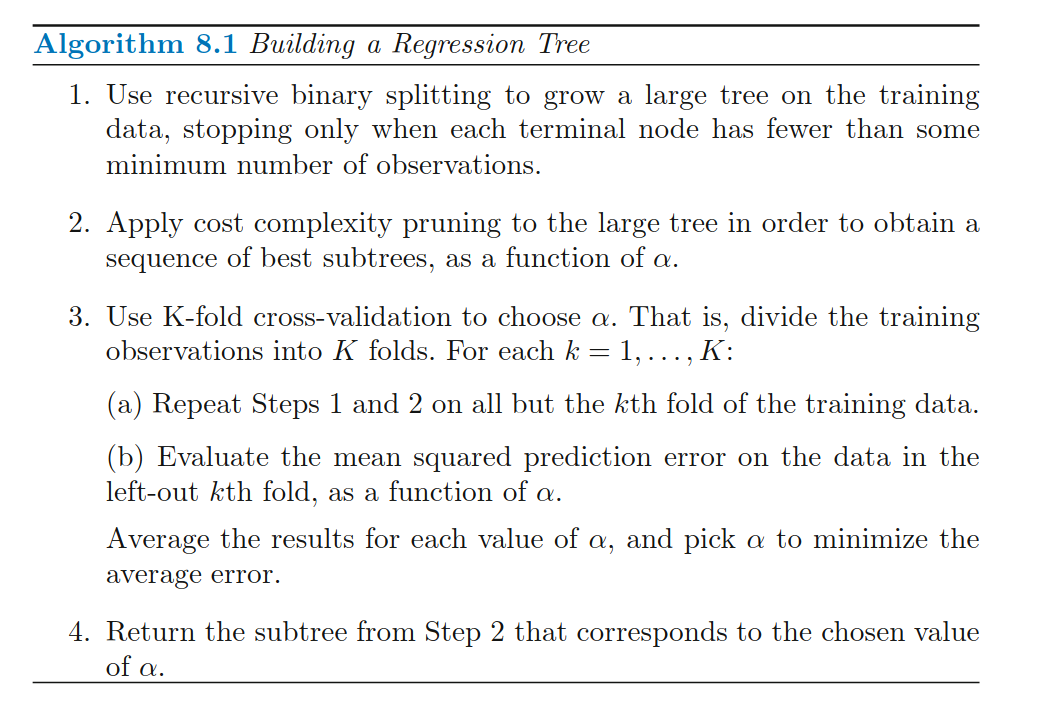
\includegraphics[height=0.9\textheight]{figs/reg_tree_estimate.png}
\end{frame}


\begin{frame}{Regressionsträd med cost complexity pruning: exempel}
    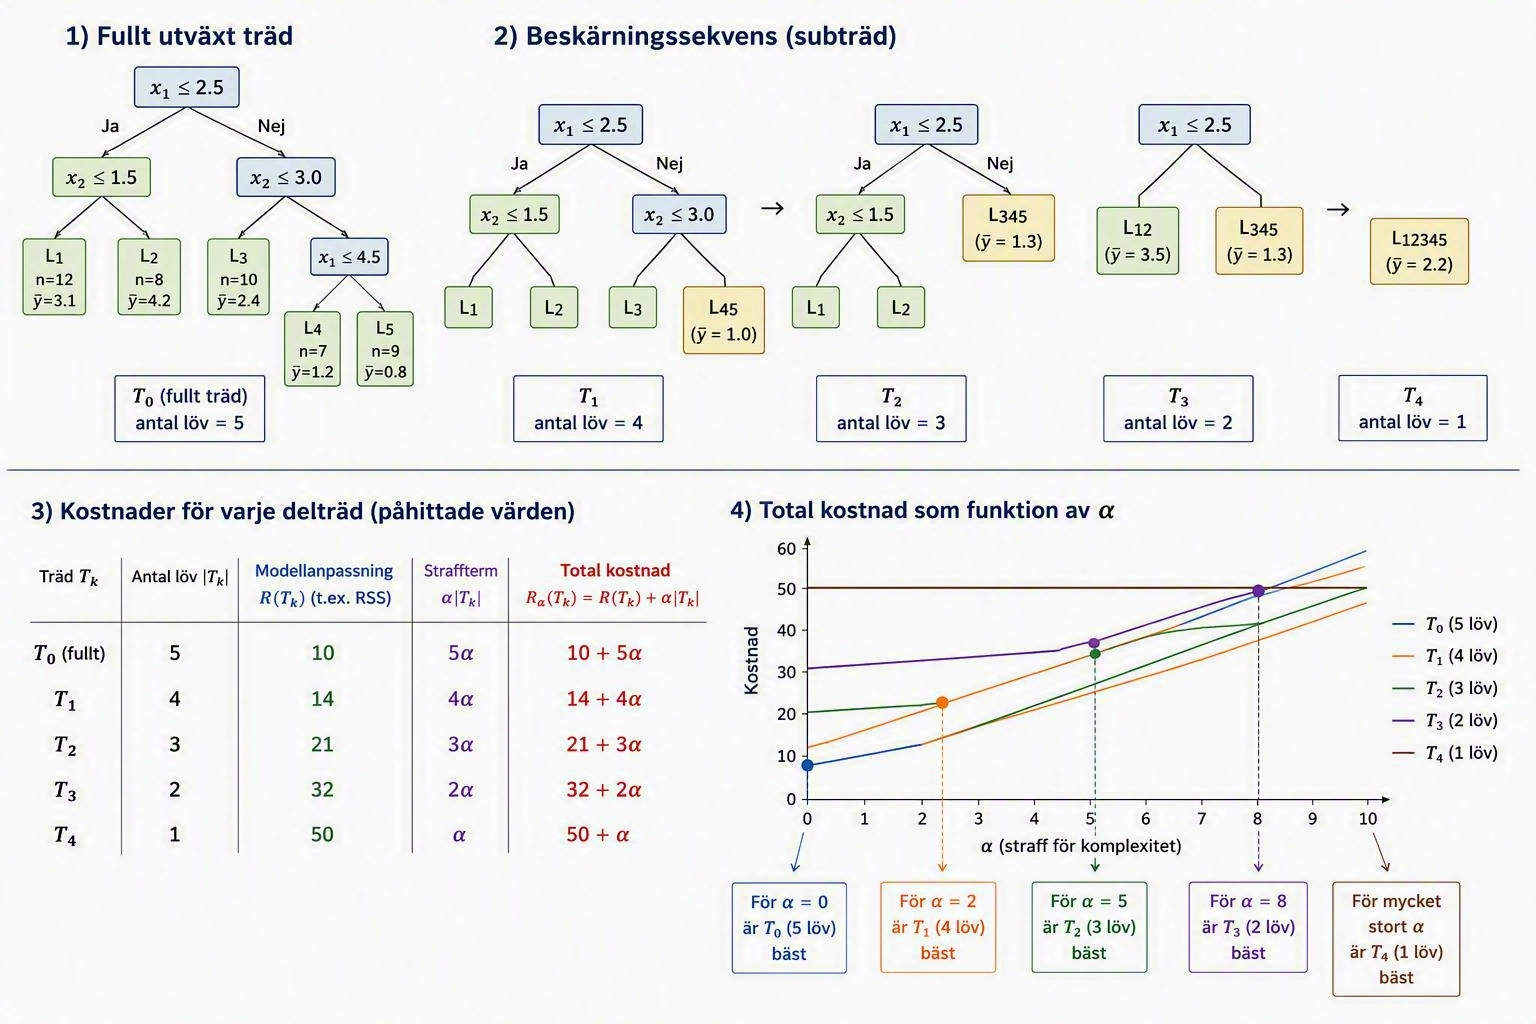
\includegraphics[height=0.9\textheight]{figs/tree_cost_complexity2.png}
\end{frame}


\begin{frame}{Trädmodell eller linjär modell}
    För regression har vi:

    \myheading{Linjär regression}
    \begin{equation*}
        f(x) = \beta_0 + \sum_{i=1}^{p} x_i \beta_i
    \end{equation*}

    \myheading{Regressionsträd}
    \begin{equation*}
        f(x) = \sum_{i=1}^{M}c_i \mathbb{I}_{c \in R_i}
    \end{equation*}
\end{frame}

\begin{frame}{Trädmodell eller linjär modell}
    För klassificering har vi:

    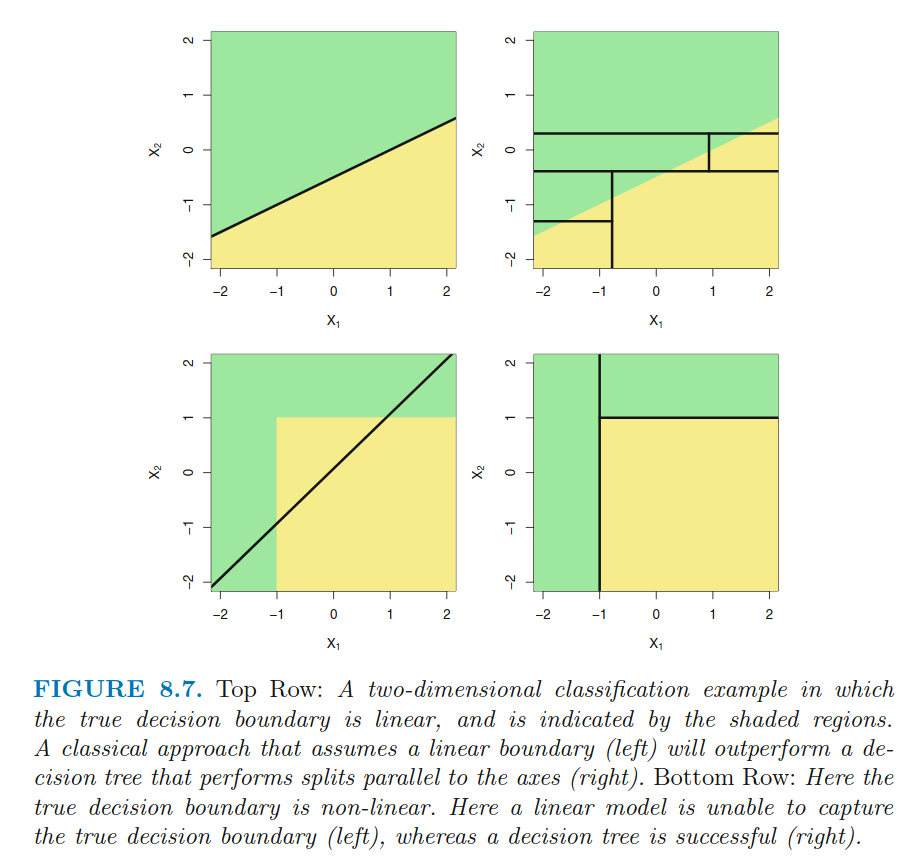
\includegraphics[width=0.68\textwidth]{figs/trees_vs_linear.png}

\end{frame}

\begin{frame}{Kommentarer om trädmodeller}
    Fördelar:
    \begin{itemize}
        \item Lätta att förstå och tolka
        \item Klarar av olika responsvariabler
        \item Kräver inte så mycket datahantering innan
        \item Funkar på relativt stora dataset
        \item Icke-parametrisk metod
        \item Automatisk variabelselektion
        \item Lär sig variabelinteraktioner automatiskt
        \item Kan anpassa många olika sorters funktioner
    \end{itemize}

\end{frame}


\begin{frame}{Kommentarer om trädmodeller}

    Nackdelar:
    \begin{itemize}
        \item Sämre prediktiv förmåga än vissa andra metoder
        \item Orubusta: överanpassar lätt
        \item Omöjligt att hitta det optimala trädet
        \item Vissa enkla funktioner kräver ett komplext träd
    \end{itemize}
\end{frame}



\begin{frame}{Kommentarer om trädmodeller}

    Förbättringar:
    \begin{itemize}
        \item Bagging
        \item Random forest
        \item Boosting
        \item BART: Bayesian Additive Regression Trees
    \end{itemize}
    
\end{frame}

\begin{frame}{Ensamblemetoder}
    
    Grundidén är att skatta många modeller på träningsdata och sen kombinera dessa för att göra prediktioner.
    
    Finns många olika varainter:
     \begin{itemize}
        \item Göra slumpmässiga urval från träningsdata och skatta modeller på dessa urval (Bootstraping/Bagging)
        \item Skapa en mängd dataset där observationerna har olika vikter i modellanpassningen i olika dataset (Boosting)
        \item Skatta ett antal olika modeller (kan vara av helt olika sort) och sen kombinera dessa vid prediktioner
        \item Vissa modeller har slumpmässiga element vid optimieringen (tänk neurala nätverk): optimera samma modell flera gånger men med olika seed, vilket ger olika modeller/parameterar. Kombinera dessa sedan vid prediktionen.
    \end{itemize}

\end{frame}


\begin{frame}{Ensamblemetoder}
    
    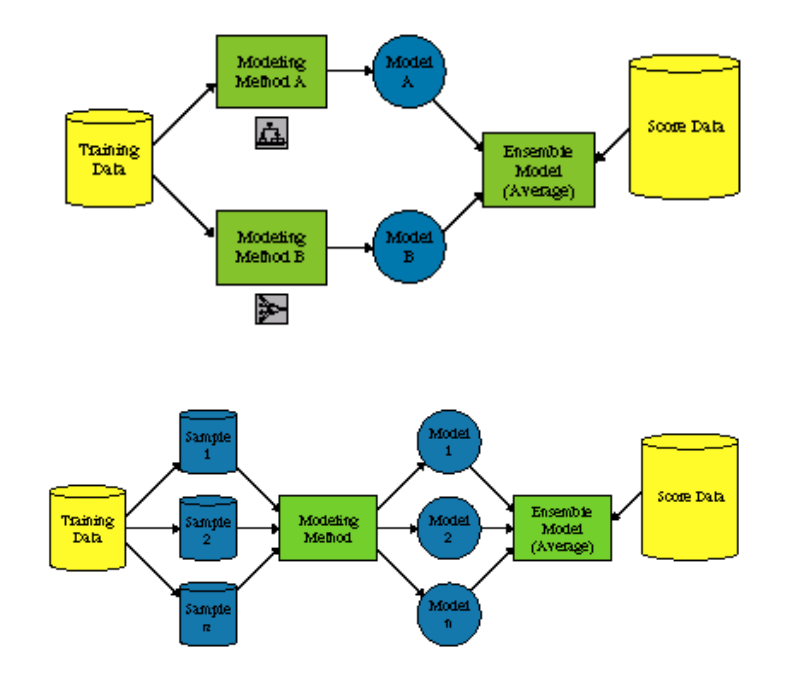
\includegraphics[width=.8\textwidth]{figs/ensample_cat.png}

\end{frame}

\begin{frame}{Bootstraping}
    
    \begin{greenbox}
        Idé: Skapa $B$ stickprov av datan genom att \textbf{med återläggning} välja nya datapunkter. Använd dessa stickprov för att skatta modell eller funktioner.
    \end{greenbox}

    Exempel:

    Vi vill skatta $\mathbb{V}(e^{\bar{X}})$.

    Skapa $B$ stickprov.

    Skatta $T_k = e^{\bar{Z}_k}$ för $k = 1, \ldots, B$.

    Beräkna $\mathbb{V}(\mathbf{T})$.


\end{frame}

\begin{frame}{Bagging}
    
    Idé: Om man tar medelvärdet av oberoende observationer (modeller) så minskar variansen.

    \begin{bluebox}
        \myheading{Bagging (Bootstrap aggregating)}: Använd Bootstrap för att skapa $B$ träningsdataset och skatta en modell $\hat{f}_b$ för varje av dessa set.

        Den slutgiltliga modellen får vi genom att ta medelvärdet av alla dessa modeller:
        \begin{equation*}
            \hat{f}_{\text{bag}}(\mathbf{X}) = \frac{1}{B}\sum_{b=1}^{B}\hat{f}_b(\mathbf{X}).
        \end{equation*}
    \end{bluebox}

    \begin{itemize}
        \item Sänker variansen av den anpassade funktionen.
        \item Påverkas \emph{mycket} av kvalitén av modellen. En bra modell blir bättre, en dålig blir sämre.
        \item För klassificering, använd majoritetsröstning.
    \end{itemize}

\end{frame}

\begin{frame}{Classification and Regression Trees (CART)}
    Vi delar upp variabelrummet genom att rekrusivt göra binära uppdelningar.

    För klassificering används vanligaste klassen, för regression medelvärdet inom regionen.

    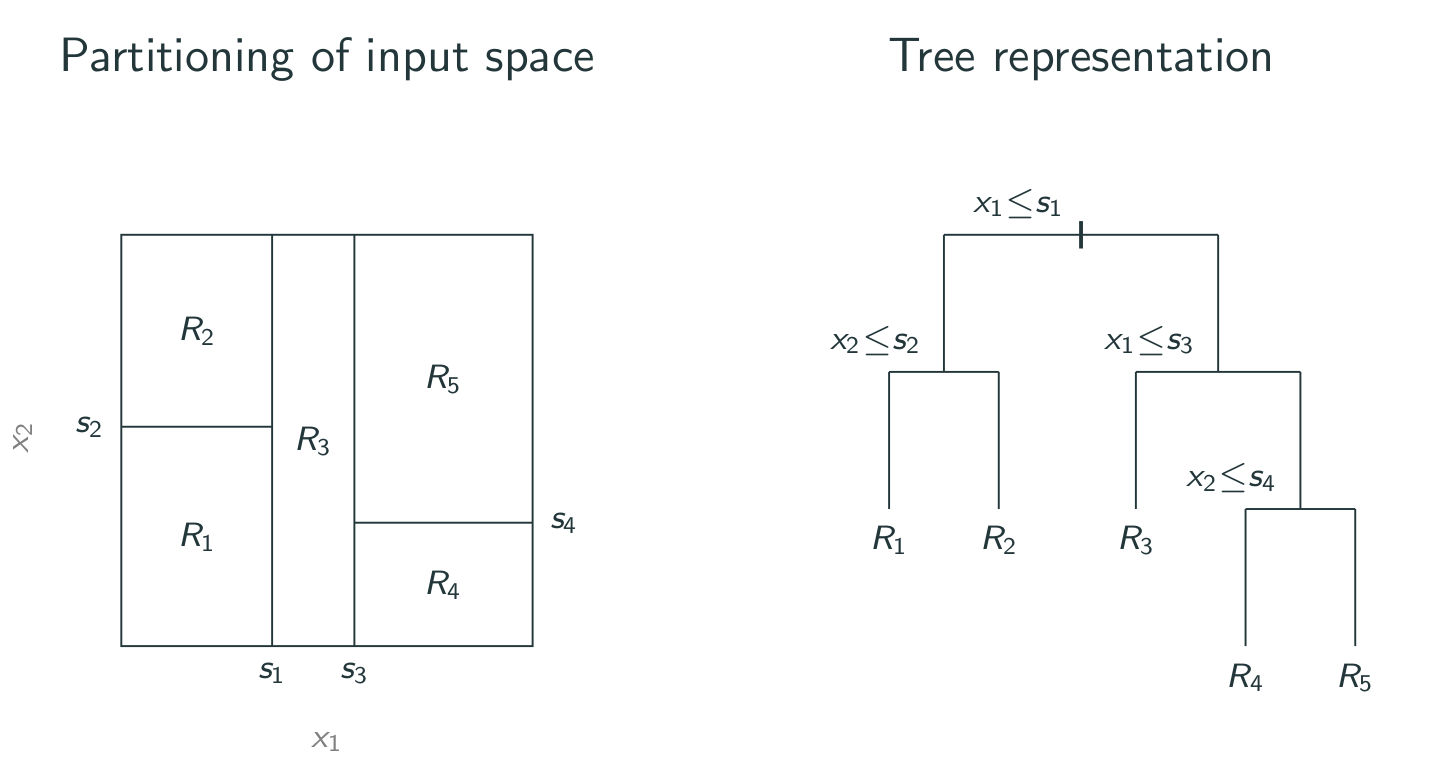
\includegraphics[width=0.8\textwidth]{figs/tree_fredrik.png}
\end{frame}

\begin{frame}{Förbättra CART}
    Flexibilitet/komplexitet för trädmodeller beror på djupet.
    \begin{redbox}
        Ett djupt träd ger litet bias, men mycket varians.
    \end{redbox}
    
    Förbättringar:
    \begin{itemize}
        \item Efterbeskärning (post-pruning):
        \begin{itemize}
            \item Skapa ett djupt träd och beskär det till ett mindre (minska variansen).
        \end{itemize}
        \item Ensamblemetoder:
        \begin{itemize}
            \item Ta ett genomsnitt över många trädmodeller.
            \item Bagging
            \item Random forest
            \item Boosted trees
        \end{itemize}
    \end{itemize}
\end{frame}

\begin{frame}{Random forest}
    
    Bagging kan ge stora förbättringar för trädmodeller. Men det finns vissa problem:
    \begin{itemize}
        \item De $B$ bootstrap-urvalen är korrelerade.
        \item Reduktionen i varians blir liten när vi tar medelvärde över korrelerade variabler.
    \end{itemize}

    Idé: Avkorrelera de $B$ trädmodellerna genom att göra slumpmässiga ändringar av modellerna.

\end{frame}

\begin{frame}{Random forest}
    
    \begin{itemize}
        \item Använd bagging för att skatta $B$ träd,
        \begin{itemize}
            \item Vid varje uppdelning/regel använd endast en slumpmässig delmängd $q \leq p$ av de förklarande variablerna.
        \end{itemize}
        \item Tumregel: (Förslag från Leo Breiman)
        \begin{itemize}
            \item Klassificering: $q = \sqrt{p}$
            \item Regression: $q = p/3$
        \end{itemize}
    \end{itemize}

\end{frame}

\begin{frame}{Random forest}
    Slumpmässigt val av variabler leder till:
    \begin{description}
        \item[-] Minskar bias, men ofta mycket långsamt.
        \item[-] Lägger till varians till varje träd.
        \item[+] Avkorrelerar träden.
    \end{description}
    Ofta dominerar den avkorrelerade effekten vilket leder till att MSE minskar på testdata.
\end{frame}

\begin{frame}{Random forest}
    Beräkningsmässiga fördelar:
    \begin{itemize}
        \item Lätt att parallellisera.
        \item $q <  p$ minskar kostanden för vaje regel/uppdelning.
        \item Inte så många hyperparametrar.
    \end{itemize}
\end{frame}



\end{document}